\chapter{Supplementary material for \cref{chapter:sd750_combined_spectrum}}
\label{appendix:chapter_combined}

\begin{figure}[htbp]
    \centering
    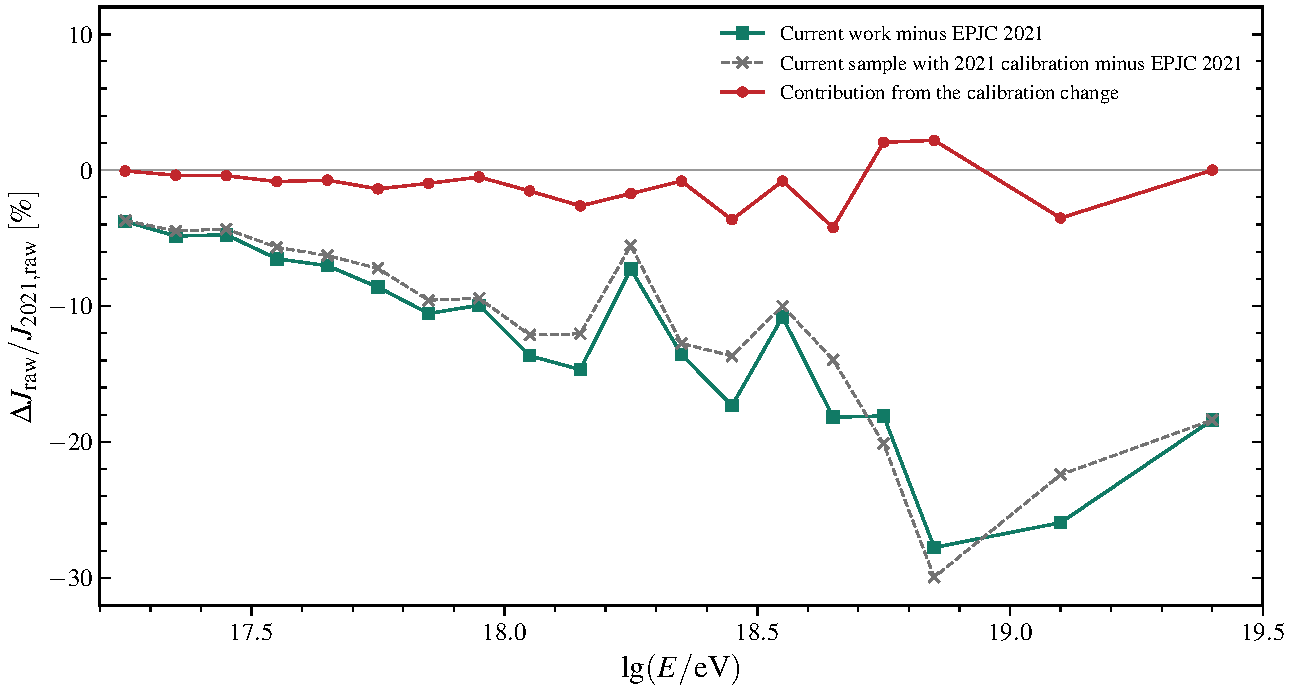
\includegraphics[width=\linewidth]{figures/chapter_combined/sd750_flux_difference_calibration.pdf}
    \caption{Relative difference between the updated raw \sd{750} spectrum and the spectrum published in 2021~\cite{PierreAuger:2021:InfillSpectrum} (green squares).
    The gray crosses show the difference obtained when the current event sample is assigned energies using the 2021 calibration relation, keeping its selection, exposure and energy bins unchanged.
    The red circles show the contribution from the calibration change, calculated as the difference between the two versions of the current spectrum.
    All differences are divided by the published raw flux, so the green values are the sum of the gray and red values.
    The calibration relations are evaluated at their nominal parameter values.
    Statistical uncertainties are not shown.}
    \label{fig:sd750_flux_difference_calibration}
\end{figure}
